\externaldocument{Introduction.tex}
\externaldocument{Experimental_Apparatus.tex}
\externaldocument{Results.tex}
\externaldocument{Analysis.tex}
\externaldocument{EIC_Jets.tex}
\externaldocument{Checks_and_Systematics.tex}
\externaldocument{Discussion.tex}

% \chapter{First Photon-Tagged Fragmentation Results in \pPb}
\chapter{Results and Discussion}

\section{Correlation Functions}
\label{sec:decaybkgsubtraction}
The final $ \gammaiso$-hadron correlations are reported in $\zt$  bins for each trigger-photon $\pt$~bin, where $\zt$~is the ratio of the associated hadron, $\pt^\mathrm{h}$, to isolated photon transverse momentum, $\zt = \pt^{\mathrm{h}}/\pt^{\gammaiso}$. The fully subtracted azimuthal correlations as a function of $ \Delta\varphi$, the azimuthal angle between the photon and the hadron, are shown in Fig.~\ref{fig:GH_Correlations} for pp and \pPb~data. With the measured \gammaiso~ constraining the parton kinematics, the distribution of away-side associated hadrons with momentum fraction \zt~represents the fragmentation function of the parton. The systematic uncertainties are discussed in detail in Chapter~\ref{sec:systematics}. The darker colored bands at zero represents the uncertainty from the uncorrelated background estimate. The vertical bars indicate the statistical uncertainty only. The final correlation functions in each collision system demonstrate similar behavior: both show a signal consistent with zero at small $\Delta\varphi$, and a rising away-side peak at large $\Delta\varphi$ arising predominantly from the hard-scattered parton opposite to the trigger photon.

 \begin{figure*}
     \centering
     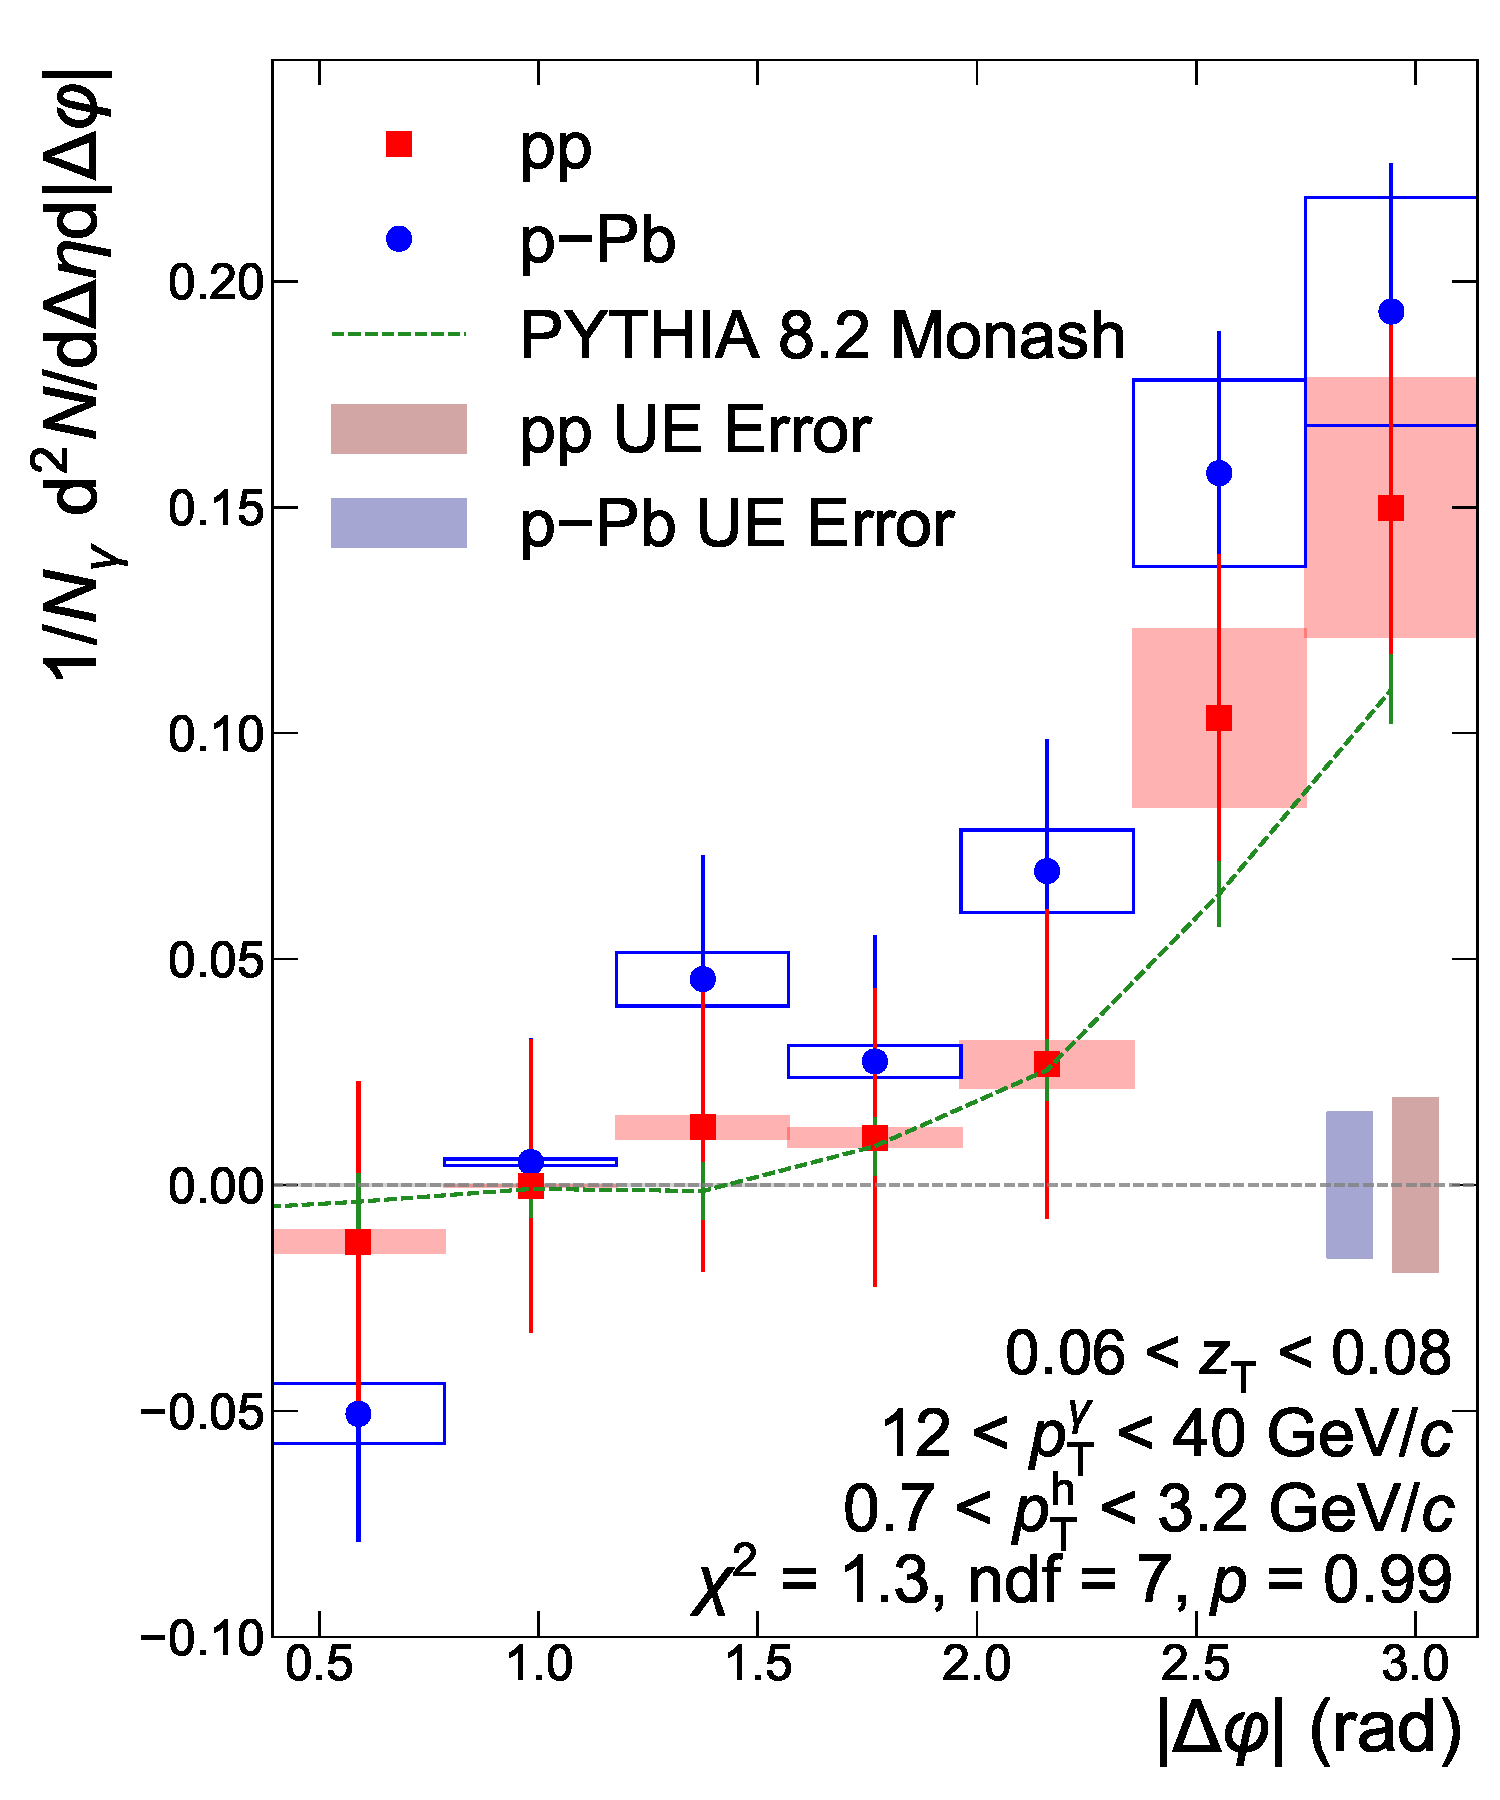
\includegraphics[width=0.3\textwidth]{Data_Analysis/gammahadron/Cs_Final_Indv_pT_0_zT_0.pdf}
    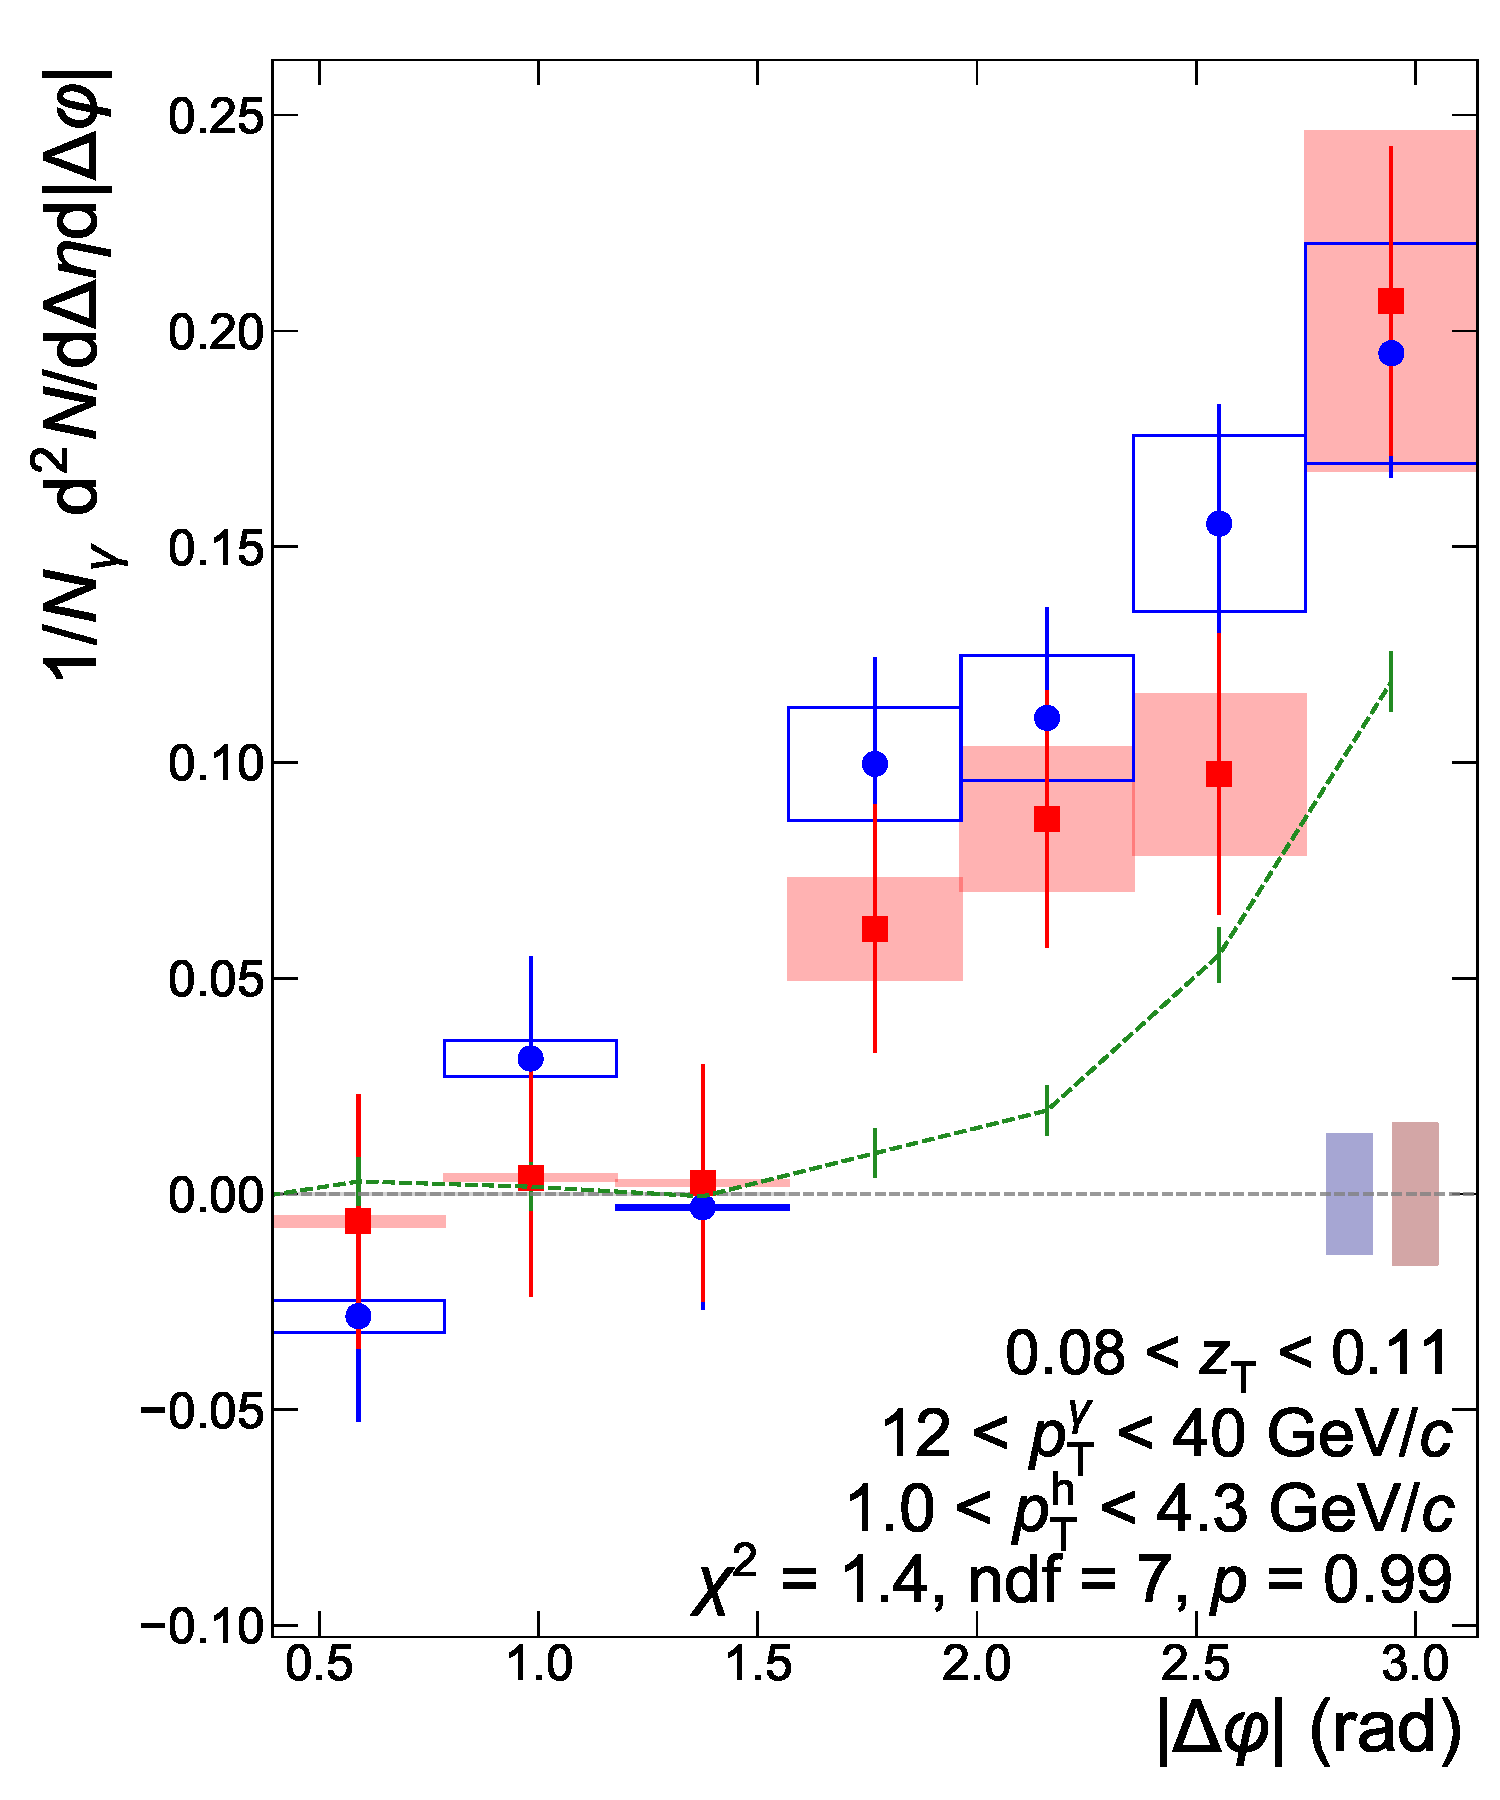
\includegraphics[width=0.3\textwidth]{Data_Analysis/gammahadron/Cs_Final_Indv_pT_0_zT_1.pdf}        
    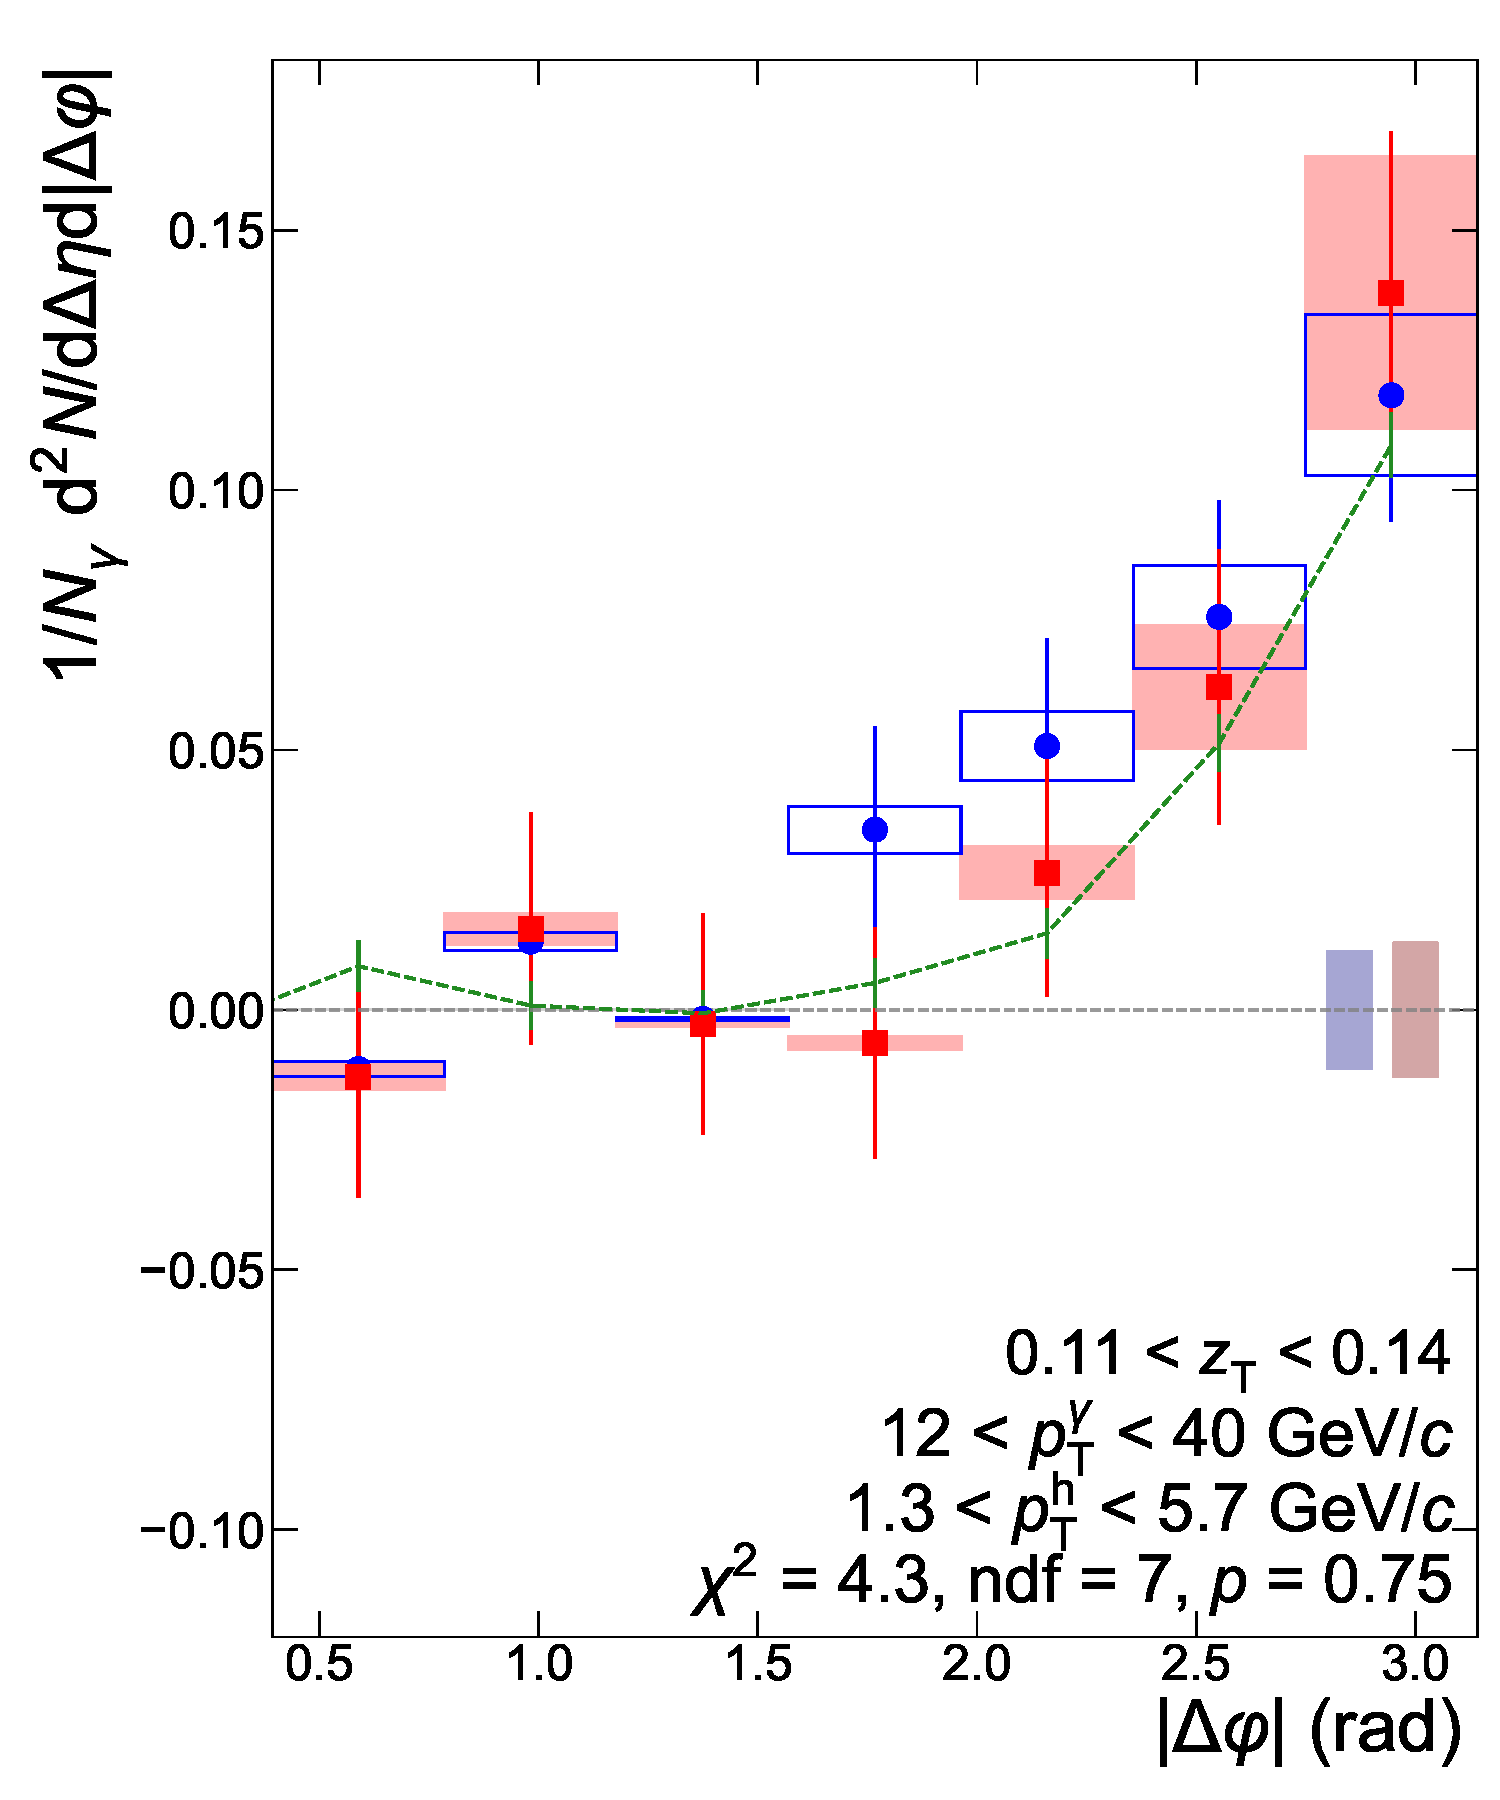
\includegraphics[width=0.3\textwidth]{Data_Analysis/gammahadron/Cs_Final_Indv_pT_0_zT_2.pdf}        
    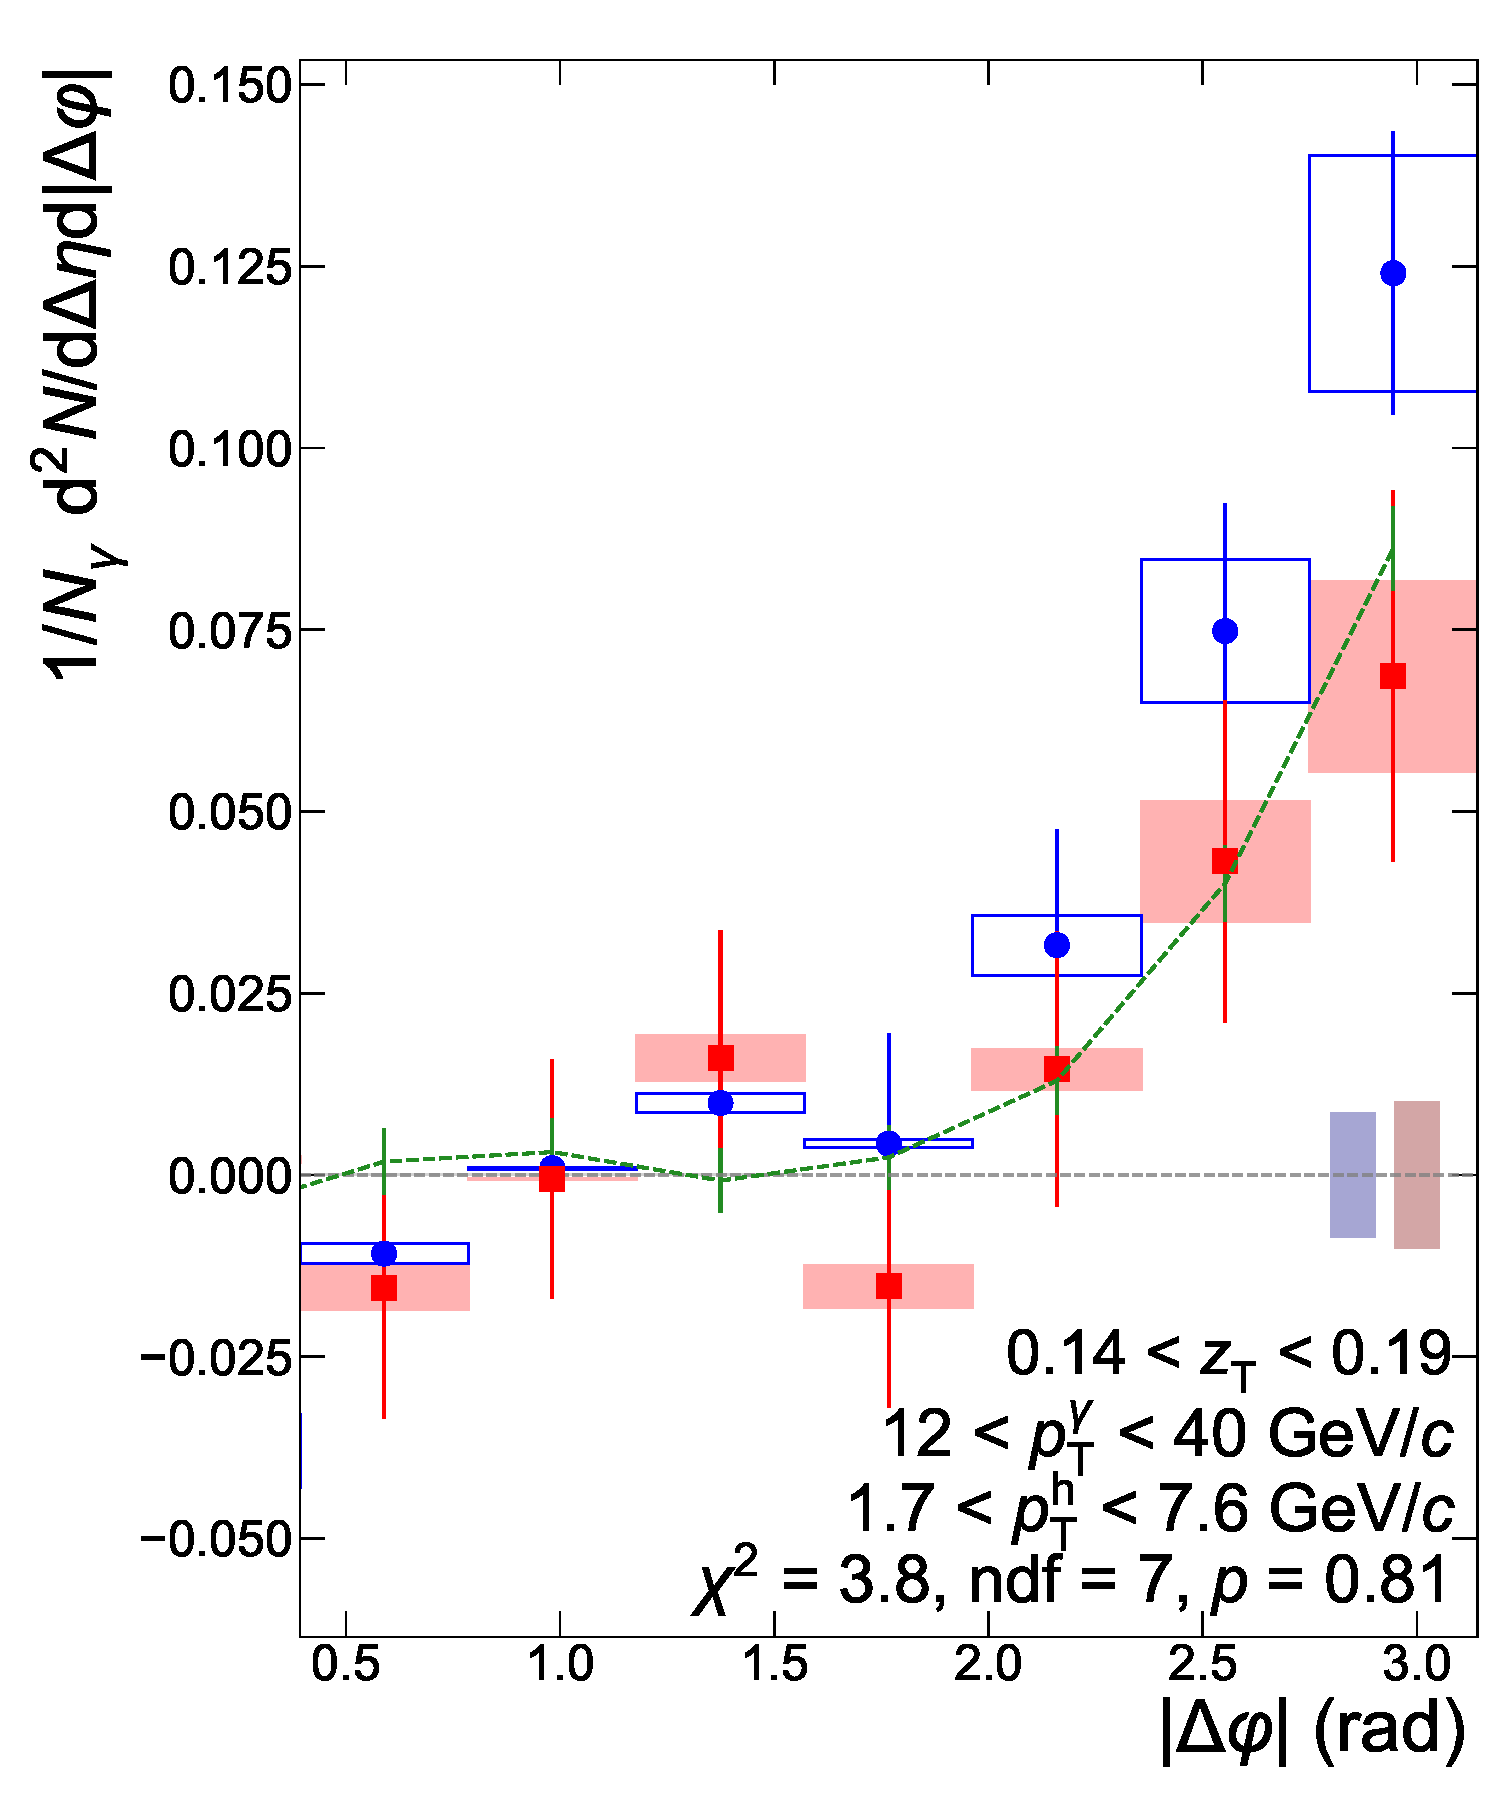
\includegraphics[width=0.3\textwidth]{Data_Analysis/gammahadron/Cs_Final_Indv_pT_0_zT_3.pdf}        
    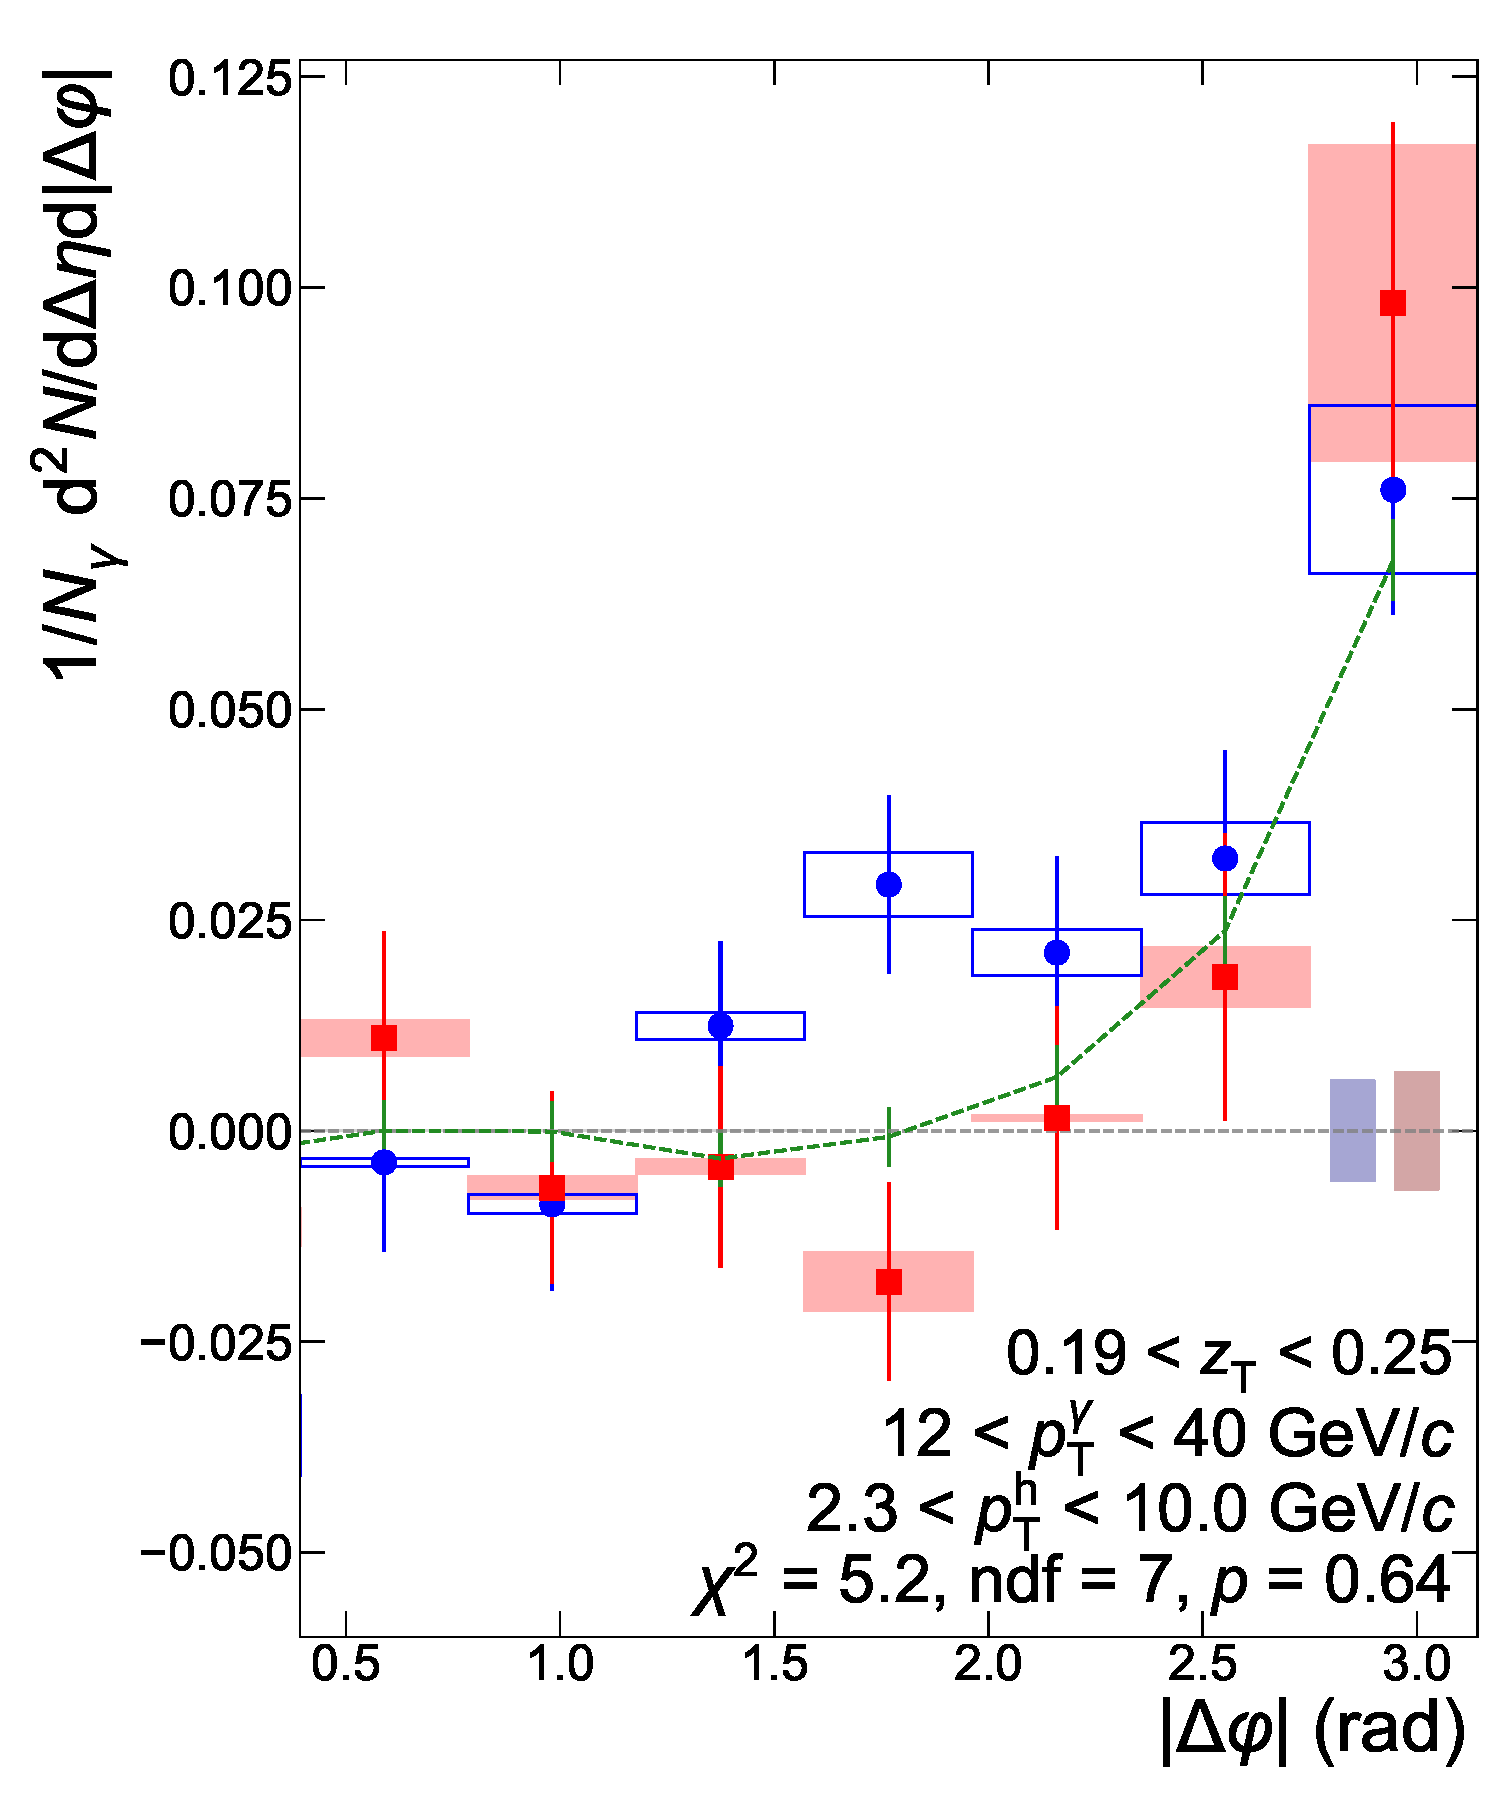
\includegraphics[width=0.3\textwidth]{Data_Analysis/gammahadron/Cs_Final_Indv_pT_0_zT_4.pdf}        
    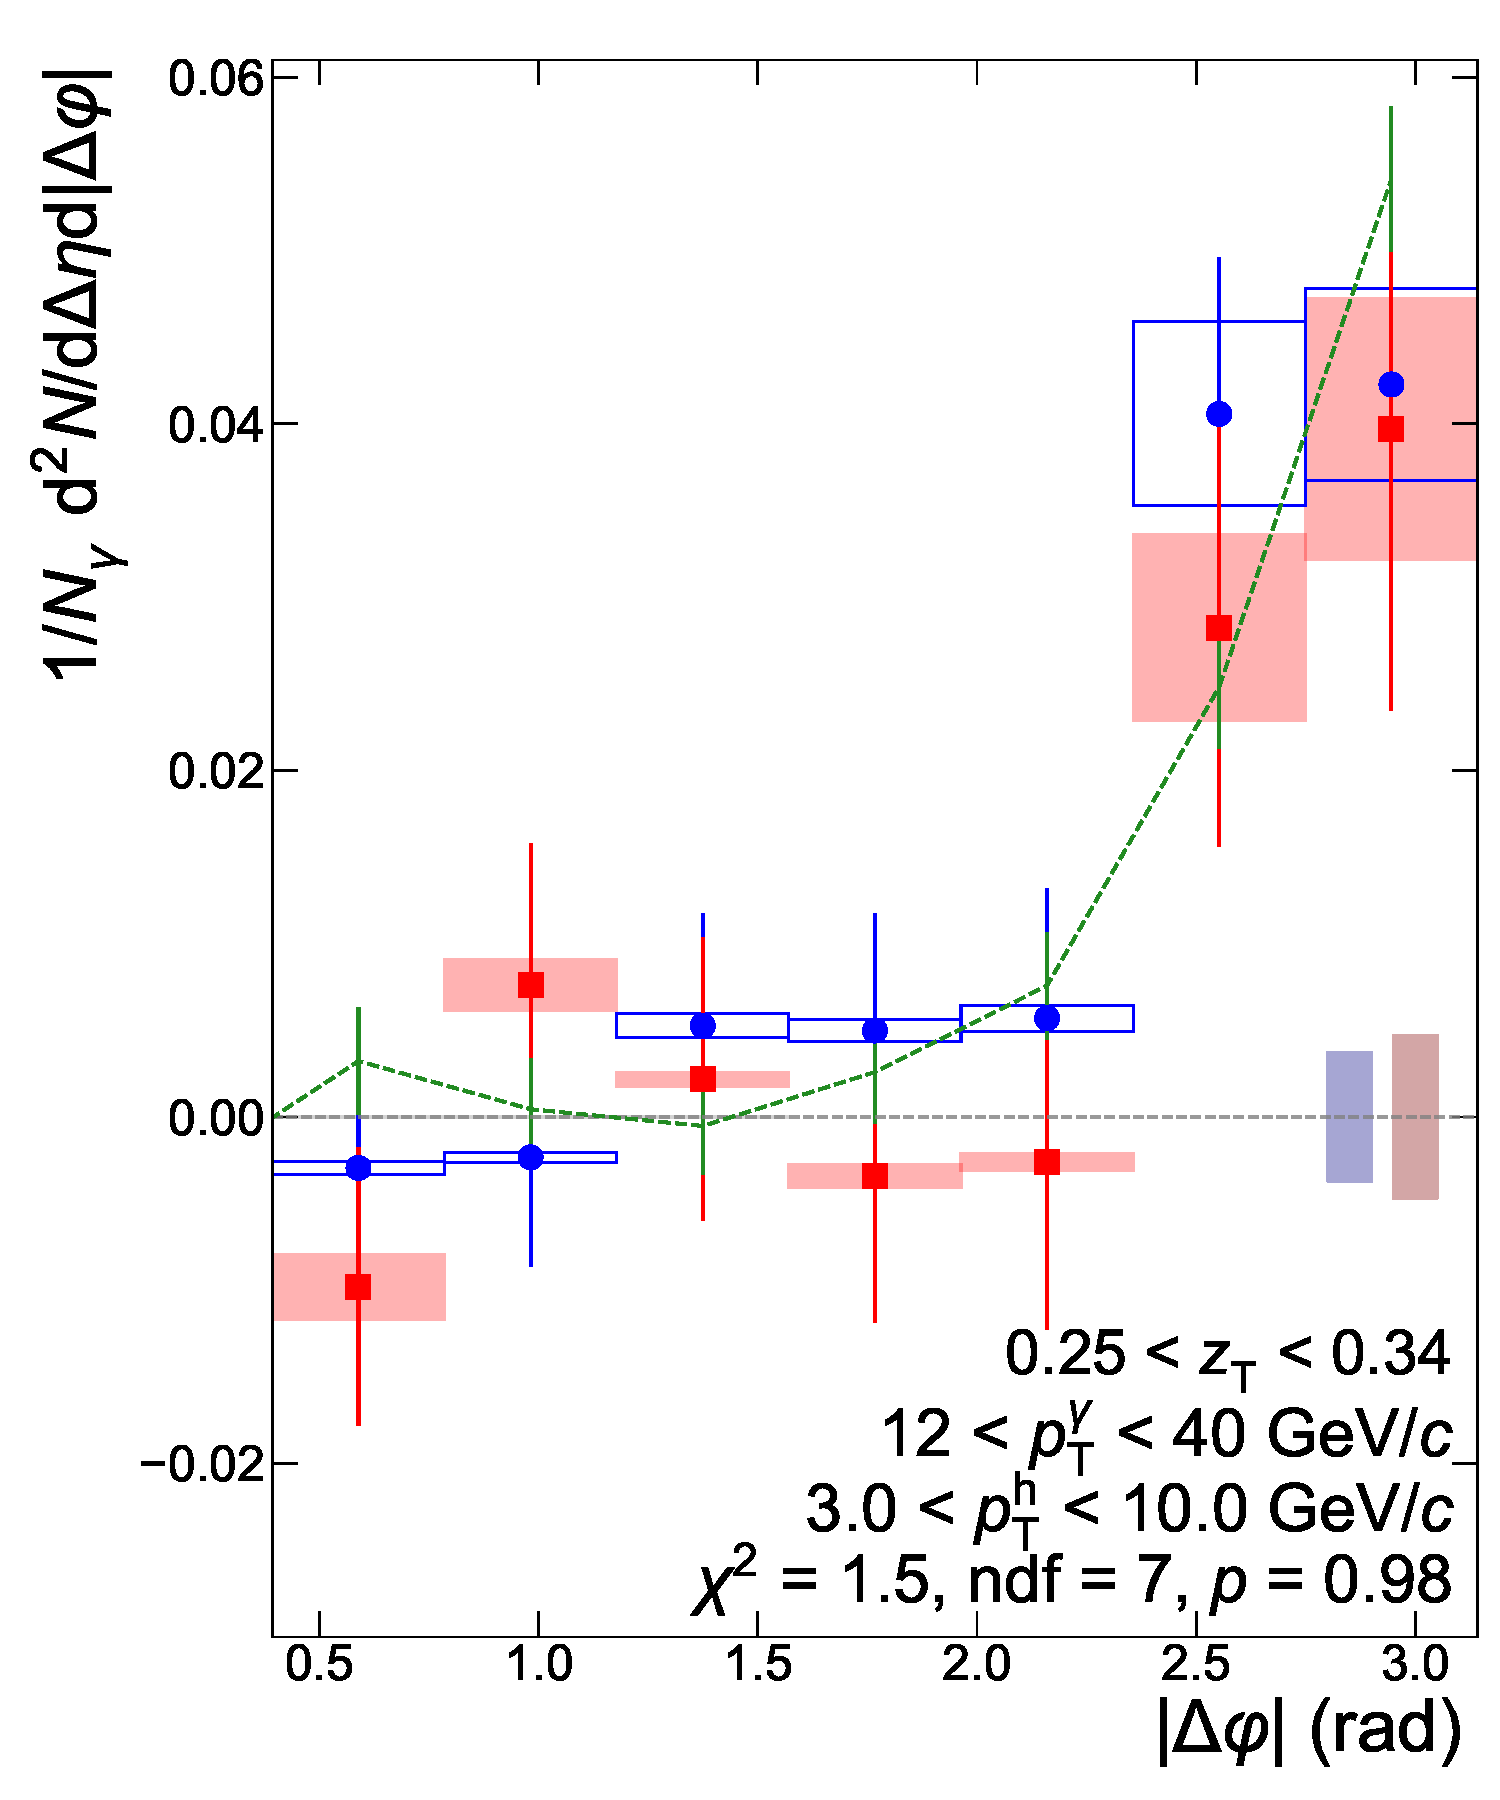
\includegraphics[width=0.3\textwidth]{Data_Analysis/gammahadron/Cs_Final_Indv_pT_0_zT_5.pdf}        
    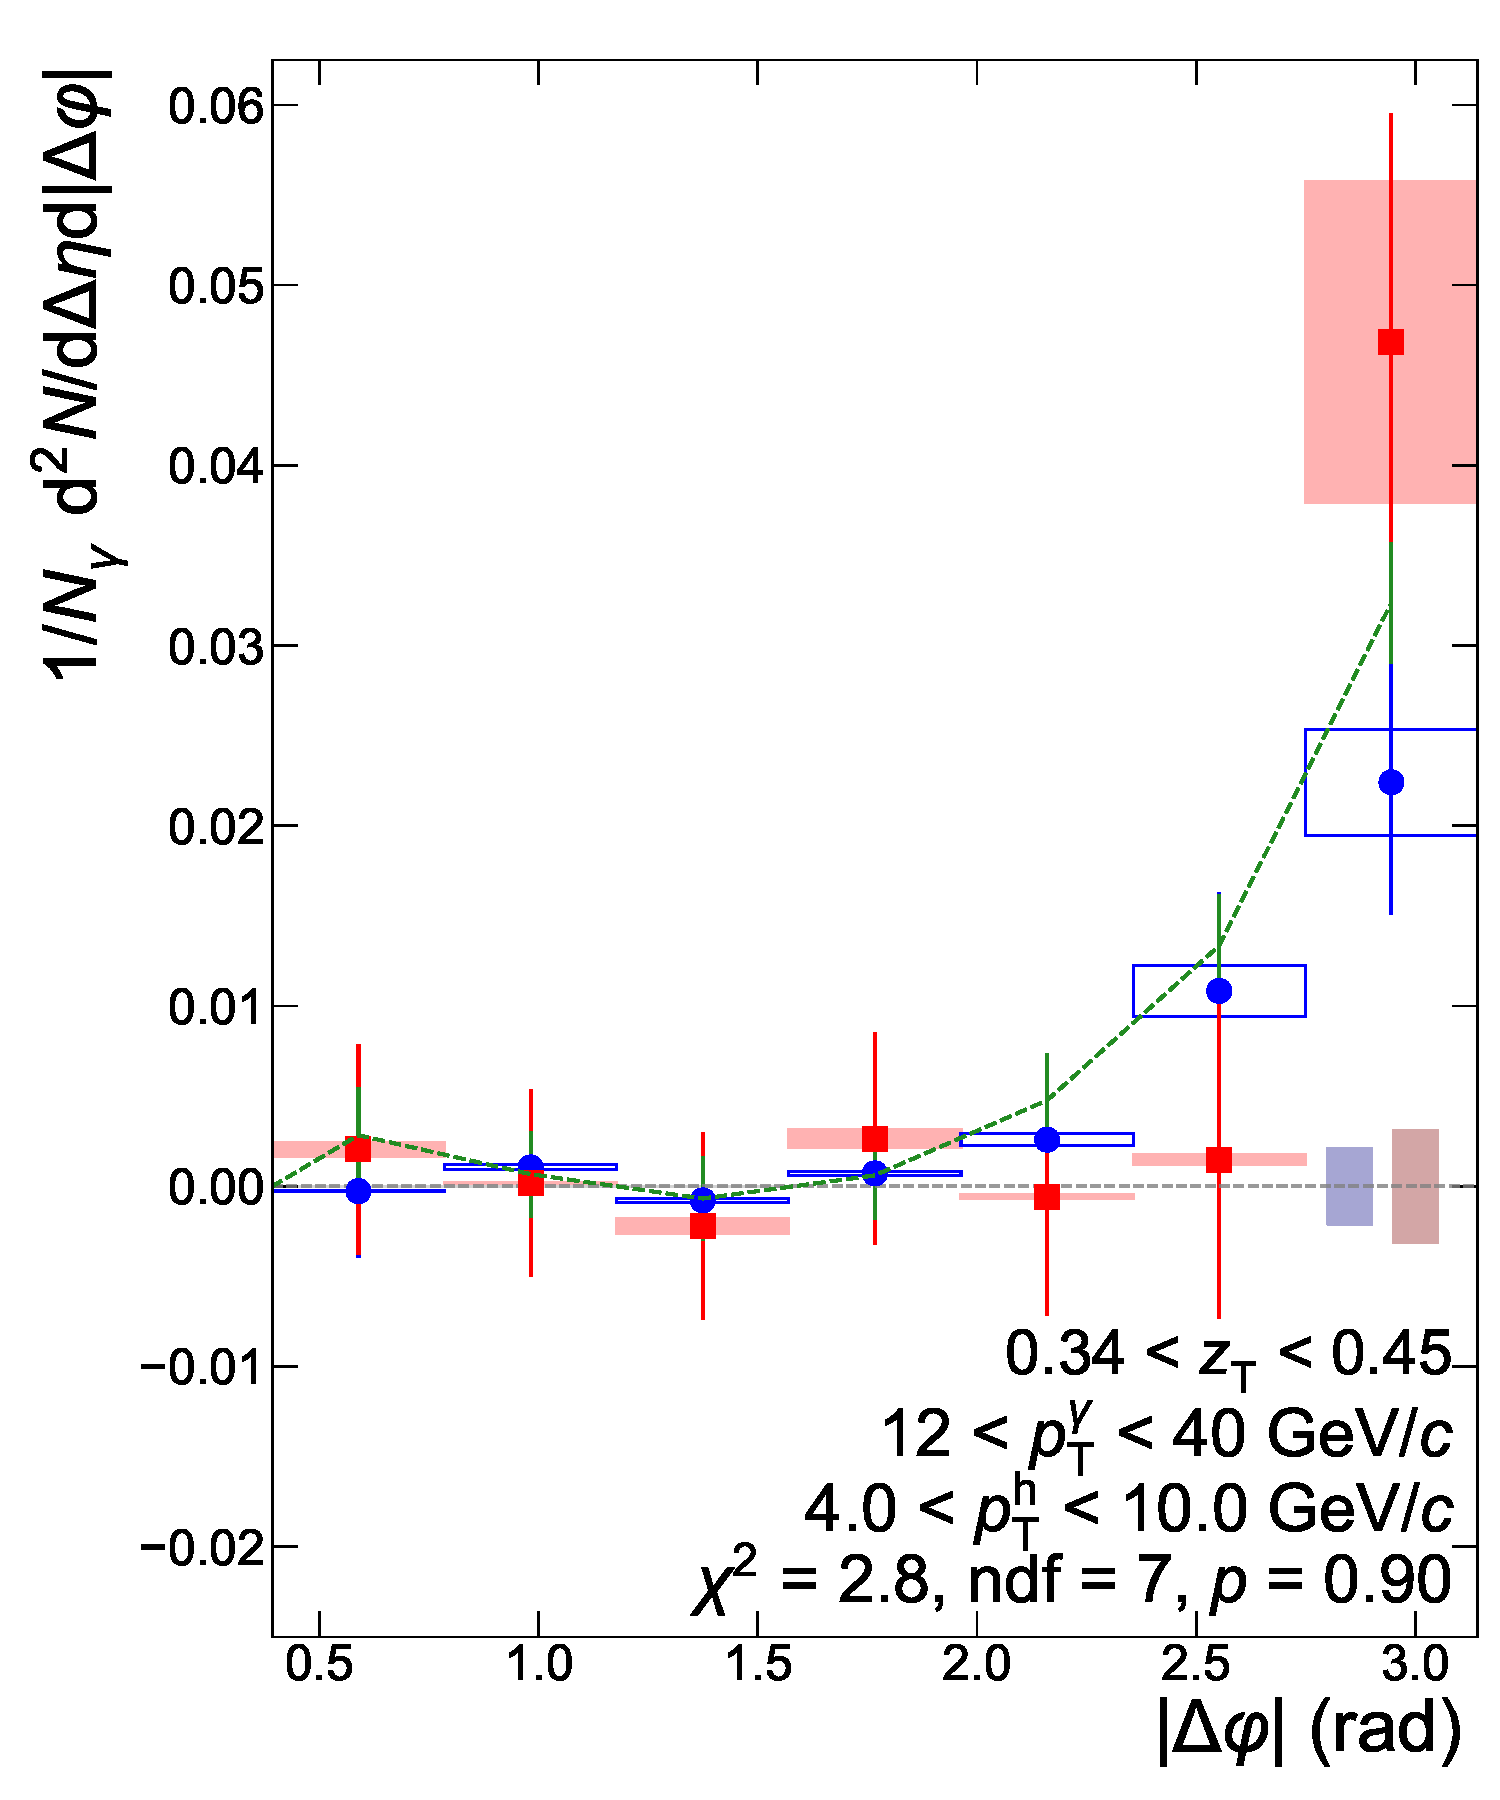
\includegraphics[width=0.3\textwidth]{Data_Analysis/gammahadron/Cs_Final_Indv_pT_0_zT_6.pdf}        
    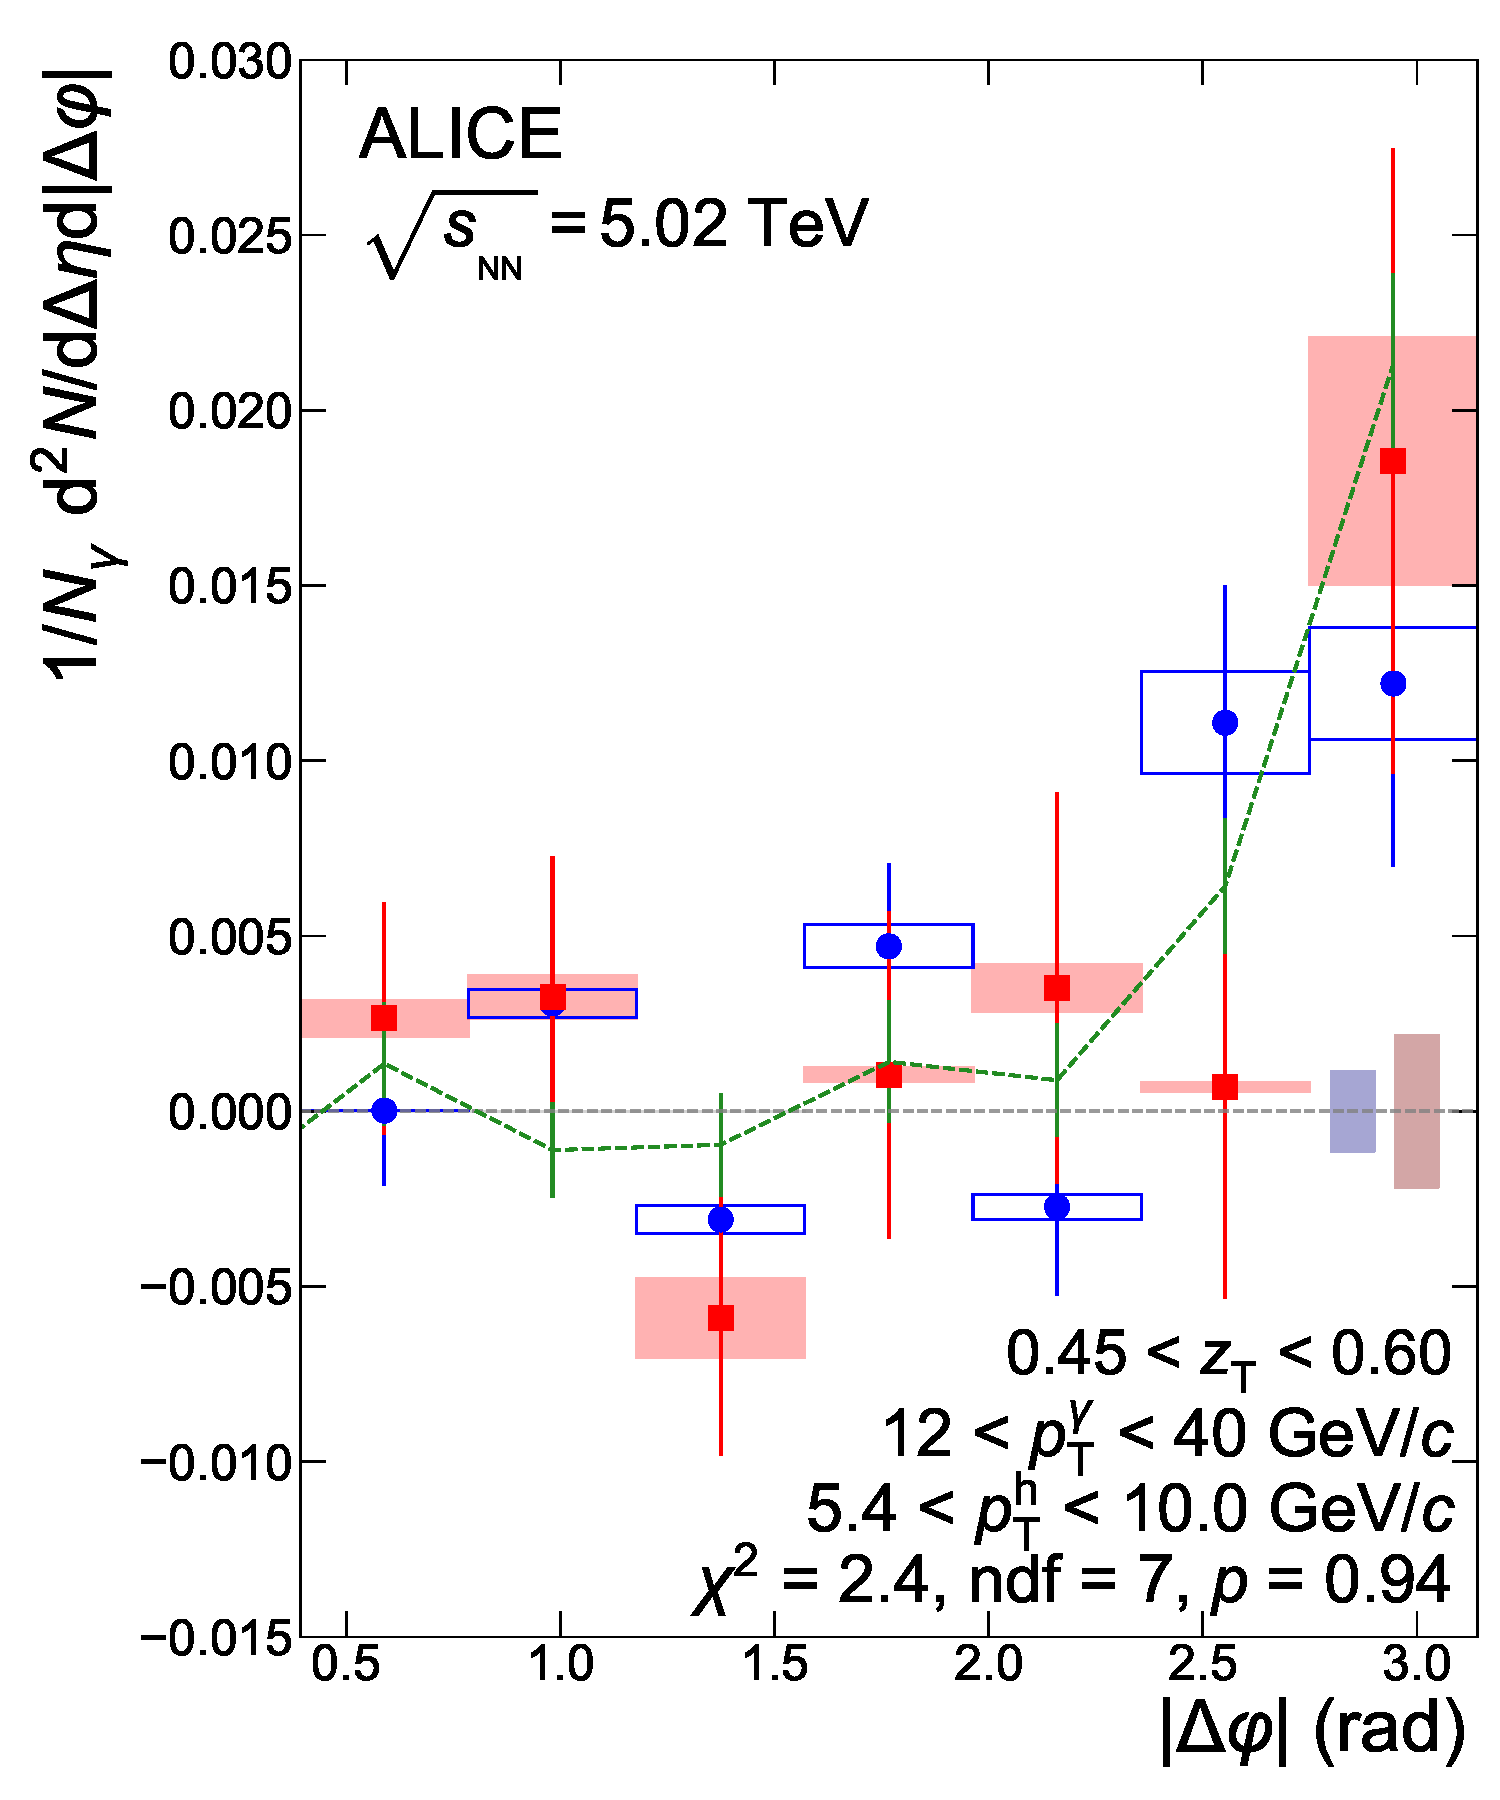
\includegraphics[width=0.3\textwidth]{Data_Analysis/gammahadron/Cs_Final_Indv_pT_0_zT_7.pdf}
    \caption{$\gammaiso$--hadron correlation functions for pp (red) and \pPb~(blue) data at $\sqrt{s_\mathrm{NN}}$ = 5.02 TeV as measured by the ALICE detector. The different panels represent three different \zt~bins. The correlation functions are projected over the range $|\Delta\eta| < 1.2$. The darker bands at zero represents the uncertainty from the underlying event estimation in pp and \pPb. The underlying event was estimated over the range $0.4 <|\Delta\varphi| < 1.6$. The vertical bars represent statistical uncertainties only. The boxes indicate the systematic uncertainties. The dashed green line represents the \gammaiso--hadron correlation function obtained with \textsc{PYTHIA 8.2} Monash Tune. ``$p$" is the p-value for the hypothesis that the pp and \pPb~data follow the same true correlation function.
    }
     \label{fig:GH_Correlations}
 \end{figure*}
\FloatBarrier

%\begin{figure*}
    %\centering
    %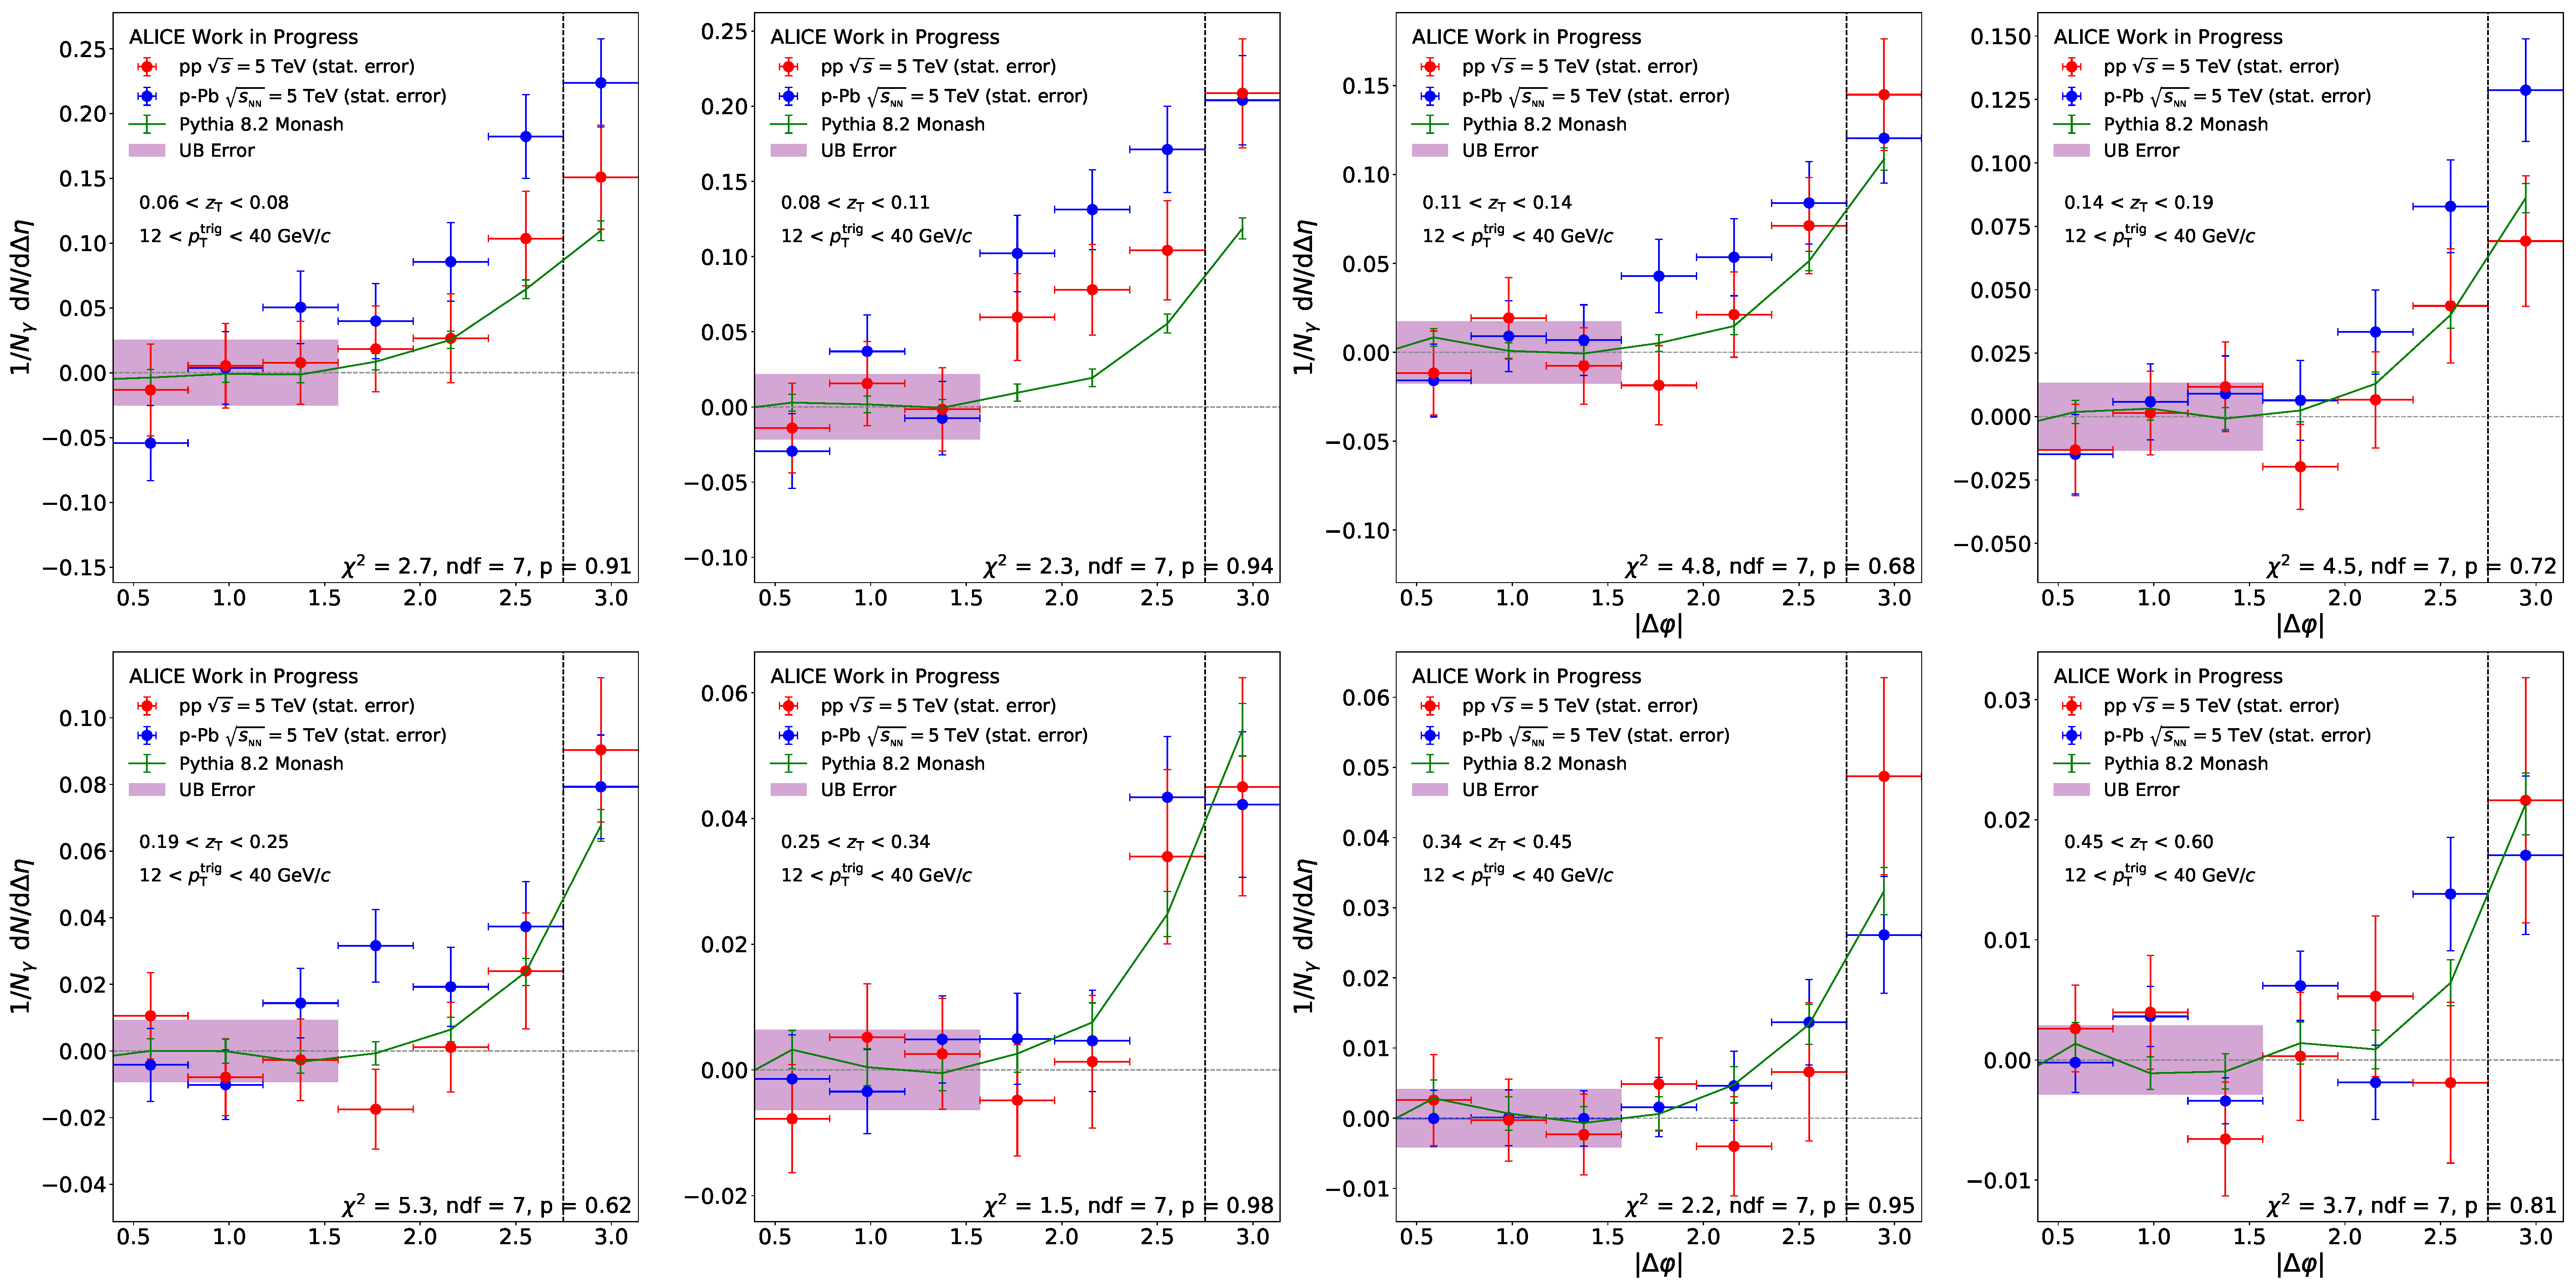
\includegraphics[width=1.0\textwidth]{gammahadron/Cs_Final_All_pT_0.pdf}        
    %\caption{$\gammaiso$--hadron correlation functions for pp (red) and \pPb~(blue) data at $\sqrt{s_\mathrm{NN}}$ = 5.02 TeV as measured by the ALICE detector. The different panels represent different \zt~bins. The purple band represents the uncertainty from the underlying event estimate n pp and \pPb. The vertical bars represent statistical uncertainty only. The horizontal bars represent the bin width in $\Delta\varphi$. The histogram is the \gammaiso--hadron correlation function obtained with \textsc{PYTHIA 8.2} Monash Tune. "p" is the p-value for the hypothesis that the pp and p-Pb data follow the same true correlation function}
%\end{figure*}

%$\gammaiso$.

Agreement within uncertainties between pp, \pPb, and the \textsc{PYTHIA 8.2} Monash Tune is observed.
By measuring associated hadrons, correlations can be observed at much larger angles than would otherwise be possible for hadrons within a reconstructed jet. A $\chi^2$ test between pp and \pPb~data and a p-value is calculated in each \zt~bin for the null hypothesis that pp and \pPb~data follow the same true correlation function. In each bin, the null hypothesis cannot be rejected, indicating that there is no significant difference between the correlation functions in the two collision systems. This conclusion is limited by the statistical precision of the available data.

\section{Parton Fragmentation Function}
As discussed in Sec.~\ref{sec:intro_gh}, the correlation functions from Fig. \ref{fig:GH_Correlations} are then integrated in the region $|\Delta\varphi| > \frac{7\pi}{8}$ for each $\zt$~bin in order to obtain the $\gammaiso$-tagged fragmentation function shown in Fig. \ref{fig:Fragmentation_Functions}. This range approximately corresponds to the azimuthal angle consistent with the commonly used radius of $R=$ 0.4 for jet measurements.

\begin{figure}
    \centering
    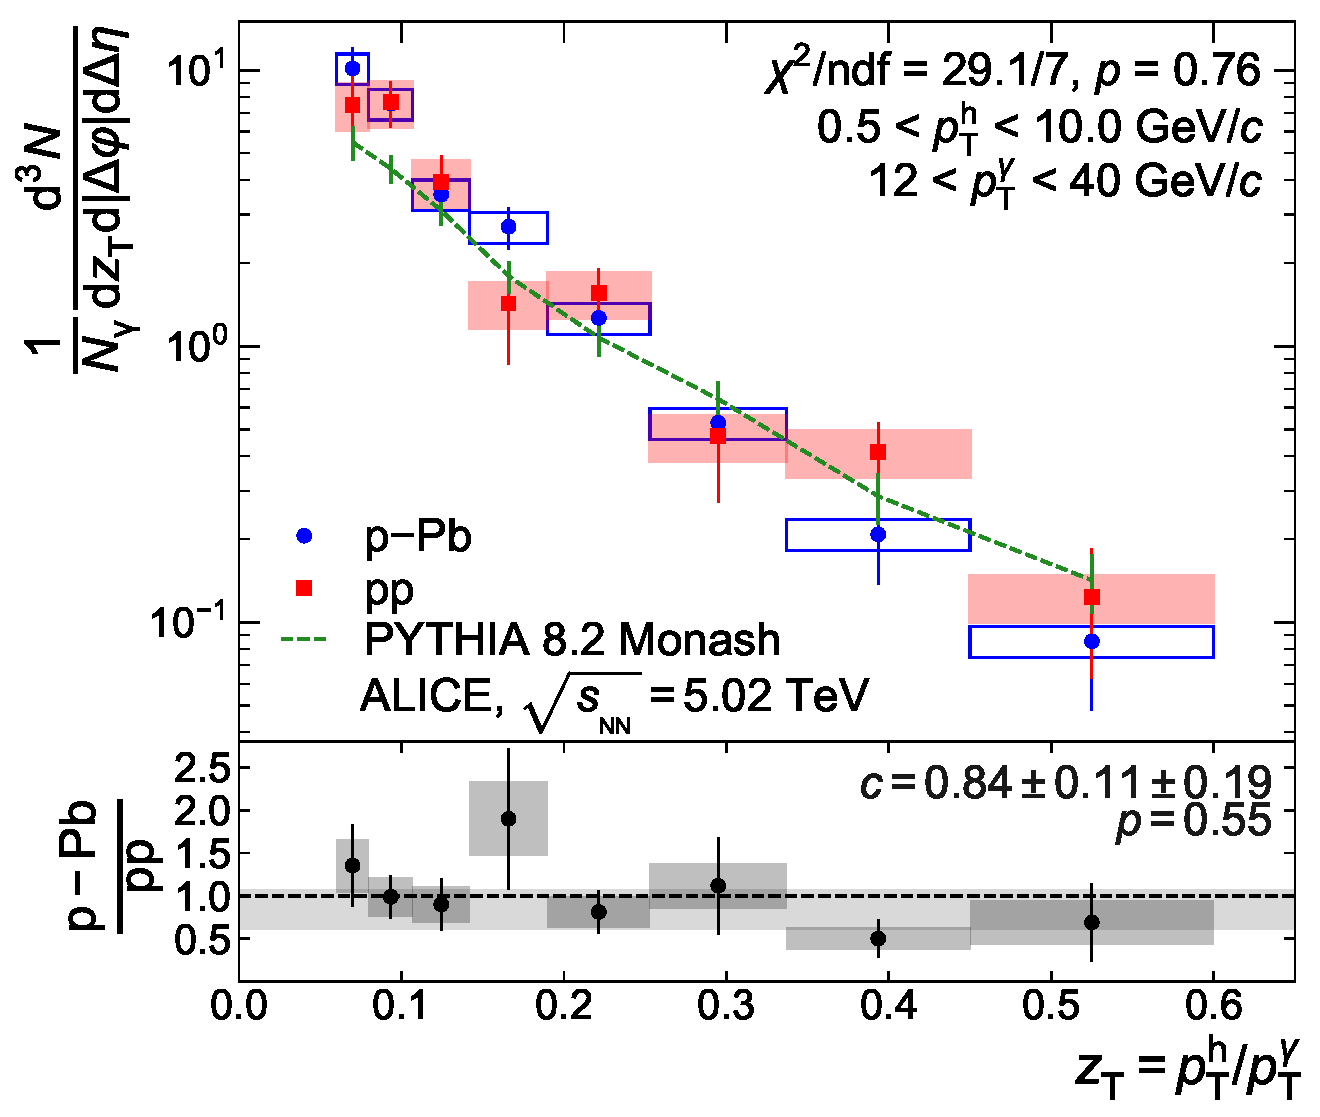
\includegraphics[width=0.67\textwidth]{Data_Analysis/gammahadron/Final_FFunction_and_Ratio.pdf}
    \caption{$\gammaiso$-tagged fragmentation function for pp (red) and \pPb~data (blue) at $\sqrt{s_\mathrm{NN}}$ = 5.02 TeV as measured by the ALICE detector. The boxes represent the systematic uncertainties while the vertical bars indicate the statistical uncertainties. The dashed green line corresponds to \textsc{PYTHIA 8.2}. The $\chi^2$ test for the comparison of pp and \pPb~data incorporates correlations among different \zt~intervals. A constant that was fit to the ratio including statistical and systematic uncertainties is shown as grey band, with the width indicating the uncertainty on the fit.}
    \label{fig:Fragmentation_Functions}
\end{figure}

The statistical uncertainty on the away-side yields in each $\zt$~bin is calculated from the statistical uncertainty in the fully subtracted correlation functions, along with the statistical uncertainty arising from the uncorrelated background subtraction. A maximum charged hadron \pt~of 10 \GeVc~and a photon trigger \pt~up to 40 \GeVc~could result in a potential bias of the associated \zt~spectrum. However, by repeating the analysis in different photon trigger \pt~bins, it was found that any such effects are negligible compared to other uncertainties. The two largest sources of systematic uncertainty are from the purity and the single track correction factors; for the chosen $\pt^{\mathrm{track}}$ interval, there is no strong $\pt$~dependence for the uncertainty of the charged tracking efficiency.

 The ratio of the fragmentation functions in \pPb~ and pp collisions is shown in the lower panel of Fig.~\ref{fig:Fragmentation_Functions}.
The fit yields a constant factor of $0.84\pm0.11\mathrm{(stat)}\pm0.19\mathrm{(sys)}$, with a reduced $\chi^{2}$ of 0.84.  
 Thus, within total uncertainties, ranging from 22--40\% for different \zt~bins the \pPb~to pp ratio is consistent with unity. %Thus, within approximately 23--40\% these uncertainties, the fragmentation function in \pPb collisions is the same as in pp collisions.

% \begin{table}
%    \centering
%    \caption{Summary of uncertainties on integrated away side yields in proton-lead and proton-proton collisions. The uncertainties quoted are absolute.} 
%    \begin{tabular*}{1.0\columnwidth}{@{\extracolsep{\fill}}llc@{}}
%     \hline
% $z_\mathrm{T}$ Range & pp $\pm$ Stat. $\pm$ Sys & p--Pb $\pm$ Stat. $\pm$ Sys. \\
% \hline
% 0.06--0.08 & 7.50$ \pm$ 2.23 $\pm$1.42 & 9.67$ \pm$ 1.82 $\pm$1.27 \\
% 0.08--0.11 & 7.66$ \pm$ 1.46 $\pm$1.46 & 7.22$ \pm$ 1.18 $\pm$0.94 \\
% 0.11--0.14 & 3.94$ \pm$ 0.96 $\pm$0.75 & 3.38$ \pm$ 0.76 $\pm$0.44 \\
% 0.14--0.19 & 1.43$ \pm$ 0.57 $\pm$0.27 & 2.58$ \pm$ 0.44 $\pm$0.34 \\
% 0.19--0.25 & 1.56$ \pm$ 0.36 $\pm$0.30 & 1.21$ \pm$ 0.25 $\pm$0.16 \\
% 0.25--0.34 & 0.47$ \pm$ 0.20 $\pm$0.09 & 0.50$ \pm$ 0.14 $\pm$0.07 \\
% 0.34--0.45 & 0.41$ \pm$ 0.12 $\pm$0.08 & 0.20$ \pm$ 0.07 $\pm$0.03 \\
% 0.45--0.60 & 0.12$ \pm$ 0.06 $\pm$0.02 & 0.08$ \pm$ 0.04 $\pm$0.01 \\
%   \end{tabular*}
%    \label{tab:FF_Summary}
% \end{table}


% \begin{table}[h]
%    \centering
%    \caption{Number of $\gammaiso$--hadron pairs per $\gammaiso$ integrated in $\Delta\varphi>7\pi/8$, for different $\zt$ intervals. The uncertainty quoted is statistical only. } 
%    \begin{tabular*}{1.0\columnwidth}{@{\extracolsep{\fill}}lccc@{}}
%     \hline
% $\zt$ range & pp & \pPb & \pPb/pp \\
% \hline
% 0.06 - 0.08 & 7.496 $\pm$ 2.230 & 9.666 $\pm$ 1.818 & 1.290 $\pm$ 0.454 \\
% 0.08 - 0.11 & 7.663 $\pm$ 1.457 & 7.216 $\pm$ 1.182 & 0.942 $\pm$ 0.236 \\
% 0.11 - 0.14 & 3.943 $\pm$ 0.959 & 3.379 $\pm$ 0.765 & 0.857 $\pm$ 0.285 \\
% 0.14 - 0.19 & 1.429 $\pm$ 0.571 & 2.584 $\pm$ 0.443 & 1.809 $\pm$ 0.786 \\
% 0.19 - 0.25 & 1.559 $\pm$ 0.356 & 1.207 $\pm$ 0.253 & 0.774 $\pm$ 0.240 \\
% 0.25 - 0.34 & 0.473 $\pm$ 0.201 & 0.503 $\pm$ 0.135 & 1.065 $\pm$ 0.536 \\
% 0.34 - 0.45 & 0.415 $\pm$ 0.116 & 0.198 $\pm$ 0.068 & 0.478 $\pm$ 0.211 \\
% 0.45 - 0.60 & 0.124 $\pm$ 0.061 & 0.081 $\pm$ 0.036 & 0.658 $\pm$ 0.434 \\
	
% \hline 
%    \end{tabular*}
%    \label{tab:ff}
% \end{table}

% Figure~\ref{ffRatio} shows the ratio of \pPb~to pp data. The systematic uncertainties in the ratio are described in Section~\ref{sec:systematics}. The uncertainty due to UE-subtraction is fully uncorrelated with $\zt$ and is combined in quadrature with the statistical uncertainty and shown as bars. All other uncertainties are correlated with $\zt$ and shown in boxes. 


% \subsection{\pPb to pp ratio}
% \subsection{Integration Window}
% \subsection{Cold nuclear matter measurements at future EIC}
% \subsection{Transverse Momentum Dependent Distributions}
% \subsection{Probing $\hat{q}$ at the EIC}
% \subsection{An All-Sillicon Tracker for Jet Measurements at the EIC}
% \subsection{Charged Jet Fragmentation Function}
% \subsection{Electron-Jet Correlations}
% \cite{Fantoni_2011}
%\section{Photon Selection}

\externaldocument{Introduction.tex}
\externaldocument{Experimental_Apparatus.tex}
\externaldocument{Results.tex}
\externaldocument{Analysis.tex}
\externaldocument{EIC_Jets.tex}
\externaldocument{Checks_and_Systematics.tex}
% \externaldocument{Discussion.tex}

\chapter{Discussion}

\subsection{Integrated Statistical Uncertainty on Fragmentation Function Ratio}
For the purpose of giving a single number to quantify how similar pp and \pPb~ fragmentation functions are, an integrated statistical uncertainty on the ratio of the two was calculated \footnote{The p-value calculated from the two distributions only indicates that the null hypothesis, pp and \pPb~ are the same, cannot be rejected}. First, the fragmentation function in pp was integrated, and the statistical errors were added in quadrature. The summed statistical uncertainty was then divided by this integral to obtain the relative uncertainty. The same was done for the \pPb~ fragmentation function. Then, the two relative uncertainties were added in quadrature and the ratio of the integrals was taken. This is shown in equation~\ref{eq:fragErrorRatio} below,

\begin{equation}\label{eq:fragErrorRatio}
\begin{split}
    I &= \sum_i y_i\cdot z_i \\
    \delta_\mathrm{abs.} &= \delta_0 \oplus \delta_1 \oplus ...\delta_n\\
    \delta_\mathrm{rel} &= \frac{\delta_\mathrm{abs.}}{I},\\
\end{split}
\end{equation}{}

where $I$ is the integral of the fragmentation function, $y_i$ is the conditional yield of associated hadrons in \zt~ bin i, and $z_i$ is the width of \zt~ bin i. Additionally, $n$ is the number of \zt~ bins, and $\delta_i$ is the statistical uncertainty of the $i_\mathrm{th}$ \zt~ bin. $\delta_\mathrm{rel}$ is the relative statistical error on the fragmentation function. Taking the ratio of the integrals and summing the uncertainties from pp and \pPb~ in quadrature:

\begin{equation}
    \delta_\mathrm{ratio} = \frac{I_\mathrm{p-Pb}}{I_\mathrm{pp}}\cdot (\delta_\mathrm{rel,pp} \oplus \delta_\mathrm{rel,p-Pb}),
\end{equation}

yields a total integrated statistical uncertainty on the ratio, $\delta_\mathrm{ratio}$ of 13\%. Thus, modifications to the fragmentation function in \pPb~are constrained to be less than 13\%.


\section{Kinematic Range Probed}

In this work, azimuthal correlations of charged hadrons with isolated photons, $\gammaiso$, are presented in \pPb~and pp collisions with a center-of-mass energy of \sqrtsNN~ = 5.02 TeV. Isolated photons are measured at midrapidity, {$|\eta|<0.67$}, and with transverse momenta in the range $12 <\pt<40$ \GeVc, which yields the scaling variable {$x_{\mathrm{T}} = 2\pt/\sqrt{s_{\mathrm{NN}}}\ = $ 0.005--0.016}. This $x_{\mathrm{T}}$ range is similar to RHIC measurements at forward rapidity~\cite{Adare:2011sc}.

This study marks the first study of photon-tagged fragmentation in \pPb~collisions at the LHC. A precise measurement of $Q^2$ in heavy ion collisions is not possible without reconstructing all particles in the event. Nonetheless, among the LHC experiments, ALICE is uniquely configured to measure low-\pt~charged particles. In the context of jet constituents and total jet \pt, ALICE is capable of measuring hard scatterings with a lower $Q^{2}$ than other LHC experiments. This is of particular interest for studying cold nuclear matter effects, as they are expected to be largest at lower $Q^{2}$. 

The agreement between pp and \pPb~in this kinematic range constrains modifications to the parton fragmentation function to be less than the integrated uncertainty of 13\% on the \pPb/pp ratio for $ 0.005 < x_{\mathrm{T}} < 0.016$, and partons with \pt~that roughly corresponds to the photon \pt~measured in this analysis.

\subsection{Insensitivity to Parton Distribution Function}
\ref{sec:FF} detailed the factorization of the hadronic cross section into the product of the parton distribution function (PDF) and the fragmentation function (FF). A very important question to answer for the study modifications to the fragmentation function in \pPb~ collisions compared to pp collisions is: How do we know if the modifications to the observed $\gamma$-tagged associated yields are due to the PDF, and not in fact modifications to the fragmentation function?

To answer this question, the prompt photon and hadronic cross sections need to be understood, and the importance of measuring  \textit{per-trigger} yields. Because the main observable is the conditional yield of hadrons per photon, modifications to the cross production cross sections cancel. Coupled with the fact the photons should not otherwise be effected by nuclear effects, this measurement is most relevant towards constraining the impact of cold nuclear modification on the parton fragmentation function. Eqn.~\ref{eq:photon_cross} shows the factorized cross sections of prompt photons in heavy ion collisions, and Eq.~\ref{eq:hadron_cross} shows the hadron cross section (shown in section \ref{sec:FF}, but displayed here again for convenience):

  \begin{equation}
    E\frac{d^3\sigma}{d^3p}(\sqrt{s},\pt) = \int dx_a \int dx_b \int dz \sum^\mathrm{partons}_{i,j}f_{i/A}(x_a)f_{i/B},(x_b) D_{\gamma/k}^{A}E_{\gamma}\frac{d^3\hat{\sigma}_{i+j}\rightarrow\gamma+X}{d^3p_{\gamma}}
    \label{eq:photon_cross}
  \end{equation}

  \begin{equation}
    d\hat{\sigma}= \sum_{a,c} \int dx_a dx_b dz f_a(x_a) f_b(x_b) d\hat{\sigma}(p_a,p_b,p_c) D_c^h(z).
    \label{eq:hadron_cross}
  \end{equation}

With $f_{i/A},(x_a)$ and  $f_{i/B},(x_b)$ being the nPDFs of the incoming partons. While the notation of the sums are slightly different, with the hadron cross section summing over flavor c, and the photon cross section summing explicitly over parton $i$ and $j$, the underlying form of the nPDFs in both equations is identical. Because this term is shared between the two cross sections, and the per-trigger yield of hadrons is proportional to the ratio of these two cross-sections, contribution from the nPDFs is cancelled for this measurement. As the conditional yield observable is directly proportional to the ratio of these two cross sections, the nPDF are not expected to contribute to the final measurement.

Thus, the answer to the question is: The observable per-trigger hadrons yields is by construction insensitive to the differences between the PDF and nPDF.

\section{Comparison to Theory}
The agreement of the ratio with unity constrains the modification of the fragmentation function to be within the reported error bars. However, careful comparison to relevant theory calculations can provide valuable insight on the specific CNM effects that are constrained by this measurement. A theory calculation on $\gamma$-hadron spectra in p+Pb for the same kinematic range as this study was performed in \cite{Xie2021}. The paper includes two models, one based on the modified nuclear PDFs, and another that simulates the formation of a small droplet of QGP in \pPb~collisions, the experimental signature of which is described in Sec.~\ref{sec:flow}. The comparison between these calculations and this measurement are shown in Fig.~\ref{fig:FF_model}.
\begin{figure}[htpb]
  \centering
  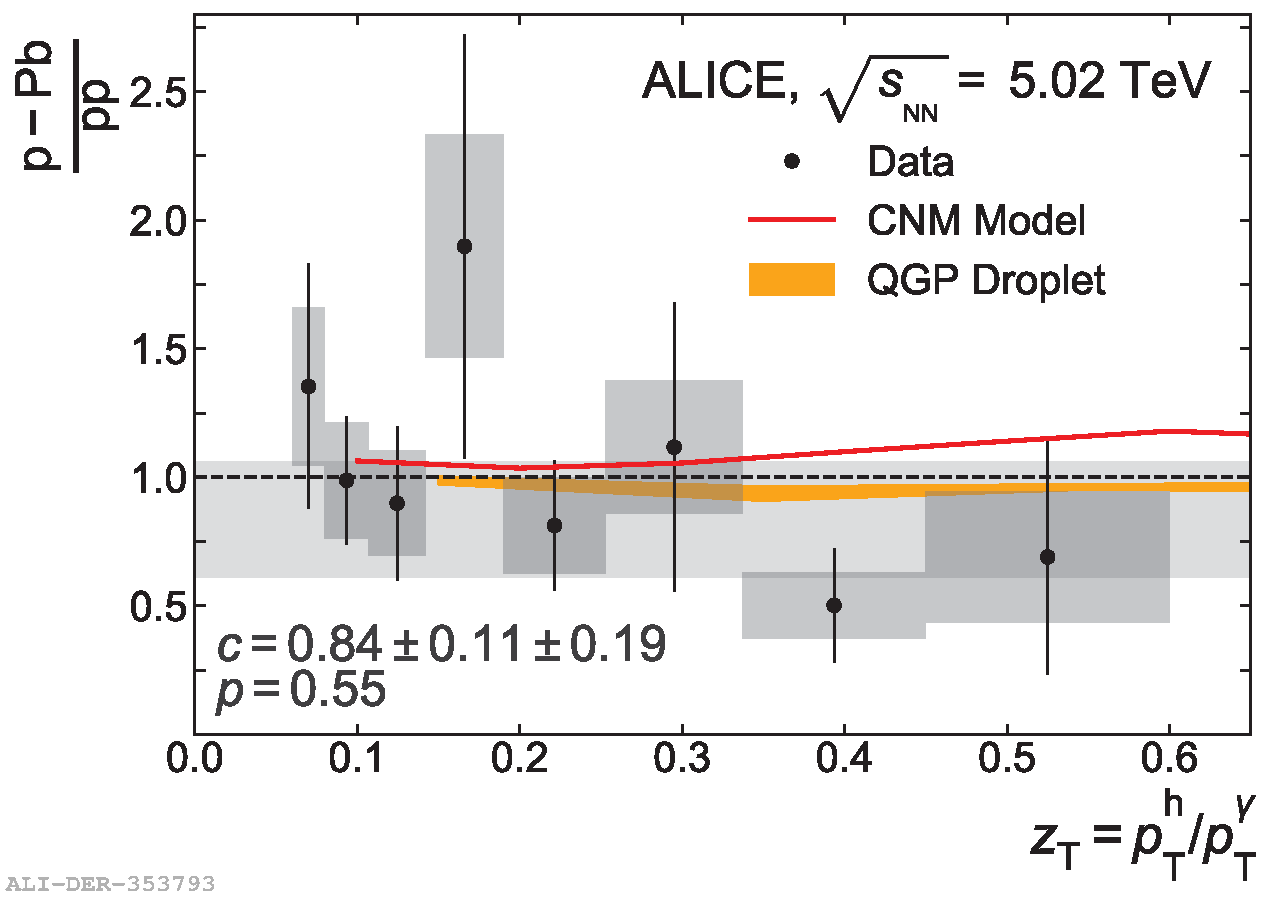
\includegraphics[width=0.8\textwidth]{FF_Model_Comparisons_Ratio.pdf}
  \caption{The ratio of isolated-tagged fragmentation functions for pp and p–Pb data at $\sqrt{s}$ = 5.02 TeV as measured by the ALICE detector.  The ratio is compared to two models from \cite{Xie2021}. The cold nuclear matter (CNM) model evolves the partons without parton energy loss, while the quark gluon pasma (QGP) model assumes that a small droplet of QGP is created in p–Pb collisions and applies an energy loss to the partons.}
  \label{fig:FF_model}
\end{figure}

Interestingly, the model predicts that even if a small droplet of QGP were to form, it's effects would be extremely small: it is closer to 1.0 in the ratio than the data, though well within the statistical or systematic uncertainties. The model involves the dynamical evolution of the QGP medium that governs the space-time evolution of the local temperature and flow velocity obtained from previous studies of jet quenching in A + A collisions, obtained using the (2 + 1) dimensional viscous hydrodynamic model with Monte Carlo-Glauber initial conditions. Qualitatively, the calculation being below unity is inline with qualitative expectations of energy loss in a QGP. While the formation of the QGP in \pPb~is currently a topic of debate in the field, this model indicates that the modification of the parton fragmentation function in \pPb~is very unlikely to unambiguously reveal it's existence. The prediction based on nuclear PDFs tells a very different story. The nuclear modification factor applied the PDFs in this model were given by the EPPS16 parametrization \cite{Eskola2017a}. It indicates that if a modification to the parton distribution function were to be observed, it should result in an enhancement at higher \zt. 

The data is consistent with both models. This is not unsurprising, despite the very different underlying physics that make up the models. This observable is designed in its inception to be insensitive to nPDFs, so any model including these effects is expected to be close to unity. As for the QGP droplet, while flow has been observed in small systems, energy loss or jet suppression has not been observed. A common explanation for the observation of flow but not energy loss is that the droplet is too small to significantly modify a parton traversing the tiny droplet. While this remains to be verified, it at least indicates that hot nuclear matter, if present at all, is expected to have a small effect on the fragmentation function. This also indicates that if a large modification were to observed in \pPb~it is unlikely to be the result of a QGP droplet.
%To measure such small modificaton to the fragmentation function in the QGP droplet scenario, significantly more precise data in pp and \pPb~ would be required.

